\documentclass{article}
\usepackage[utf8]{inputenc}
\usepackage{amsmath}
\usepackage{amssymb}
\usepackage{enumerate}
\usepackage{parskip}
\usepackage{graphicx}
\graphicspath{ {./samples/final/} }
\usepackage{biblatex}
\addbibresource{final-references.bib}

\newcommand*{\Pn}[1]{\left( #1 \right)}

\DeclareMathOperator{\Tr}{Tr}

\title{Matrix Bubbling}
\author{Adam Busis, Jacky Lee}
\date{December 17, 2018}

\setlength{\parskip}{12pt plus 1pt minus 1pt}

\begin{document}

\nocite{*}

\maketitle

\section{Abstract}

Matrix bubbling is a useful technique for analyzing big data sets because it collapses the large amount of data given into a smaller matrix of summary statistics, which is easier to work with. In this paper, we discuss matrix bubbling in two dimensions but this technique can be easier extended to higher-dimensional space.

\section{Background}

When working with big data, it often takes a long time to process data since there is so much of it. To try to resolve this problem, we want to be able to somehow reduce this data into its essence such that we numerically have less data to work with, which means we can process it faster, but still have sufficient information to extract something meaningful out of it.

One method that does this is called dimension reduction. The general idea of dimension reduction is that we can reduce the number of variables involved in our data such that we have less to work with but still enough information to perform computations with. Dimension reduction is a useful tool that enables us to analyze big data sets with less computation time.

Generally, this is done by determining which features define the data the most and restricting our attention to those few features. For example, consider the scenario where we want to read characters off of hand-drawn maps. Given a random symbol from the map, how do we determine whether the symbol is a letter or just some junk from the map? There can be a lot of information hidden within each symbol. One thing we could do is to only consider specific features that seem to be the most important for determining whether a symbol is a letter or not. For example, we can only look at the width, height, and density of the input and from there guess whether the symbol is a letter or not. This is plausible because letters on a map generally are within some size limit; they are probably not too big (taking up a quarter of the map) and they are probably not too small (taking up just 3 pixels worth of space).

Another thing that can be done is to define new features that can be thought of as combinations of multiple features. For example, we could replace our width and height feature for a new perimeter feature, which is computed by taking the sum of the width and height then multiplying by 2. We see that this perimeter feature is a combination of both the width and height features.

Currently, the main dimension reduction technique is called Principle Component Analysis, or PCA for short. Essentially, this method takes in data and computes the most important features that help identify the data.

\section{Motivation}

Let us restrict our attention to the two-dimensional case for now since it is easier to visualize. Suppose we have a large set of data distributed in two-dimensional space in a fashion that is not Gaussian. For example, the pixels representing the letter `A' are not distributed normally. Now suppose we would like to compare it with another data set that is also large and distributed in some space. Let's call these two data sets $A$ and $B$. One way to do it is to take each data point's location in the space and compare it to the analogous space in the other data set. This requires going through each point and requires a lot of computations.

The idea behind matrix bubbling is that we can somehow summarize each data set using some proxy such that if we want to compare two data sets $A$ and $B$, we can simply compare their proxies, $A_p$ and $B_p$, where the proxies are much smaller than the original data sets. The ``proxy'' can be any smaller set of data depending on the data set. This can be thought of as a sort of dimension reduction since we are reducing the amount of data we need to consider and instead summarizing the data using a few key statistics. Ideally, the proxies for two different data sets will be close together if (and only if) the two data sets are similar, where similarity of the data sets is a criterion that depends on the application.

One possible way of summarizing the data would be to look at summary statistics for the entire data set, such as the mean and variance. The problem with this method is that just the mean and variance for the entire data set don't have enough information to capture the nuances of the data set. The key idea is that we can view our space as a grid and partition this grid into smaller grids. Then for each grid, we can find a probability distribution that summarizes the data within that grid and use it as a proxy. Since probability distributions can be summarized by a few statistics such as the mean and covariance for a Gaussian distribution, this reduces the number of data points we have to consider. By changing the number of smaller grids (and therefore the size of the smaller grids) that we divide the data set into, we can adjust the fineness of the details we look at in the data based on the application.

\section{Introduction}

Suppose we have a matrix $M$ representing a two-dimensional data set which we would like to compare to another matrix $N$ representing a different data set. To do this comparison, we would want to use a metric. Some of the available options for this include Euclidean distance, $L_p$ norms, etc. Any of these will work fine if our data set was small. But what happens when the data sets get very large? Pairwise distance metrics get very difficult to compute, and biases become able to skew the distances off significantly. Because of how applicable big data is, these are often the scenarios we run into the real world.

To solve this problem of comparing two matrices $M$ and $N$ representing two dimensional data sets, we propose matrix bubbling.\cite{gu}

The first step to matrix bubbling involves summary. The goal of summary is to make the large data set finite and computationally small while retaining all the essential features of the data set. Summary sets out to transform the original $m$ by $m$ matrix where $m$ is significantly large to an $n$ by $n$ matrix where $n$ is computationally small. As this point, one might start to wonder - how large is significantly large and how small is computationally small - and the answer to this is - it depends. It depends on the data set and the application for which the data sets are used. In our tests of this approach, we transform high quality images of about $1920 \times 1024$ to low quality images of about $288 \times 288$. Once the dimensions have been chosen, the goal would be to divide the original $m$ by $m$ matrix to square grids of size about $\frac{m}{n}$. A pictorial representation of this has been put below.

\begin{figure}[h!]
\begin{center}
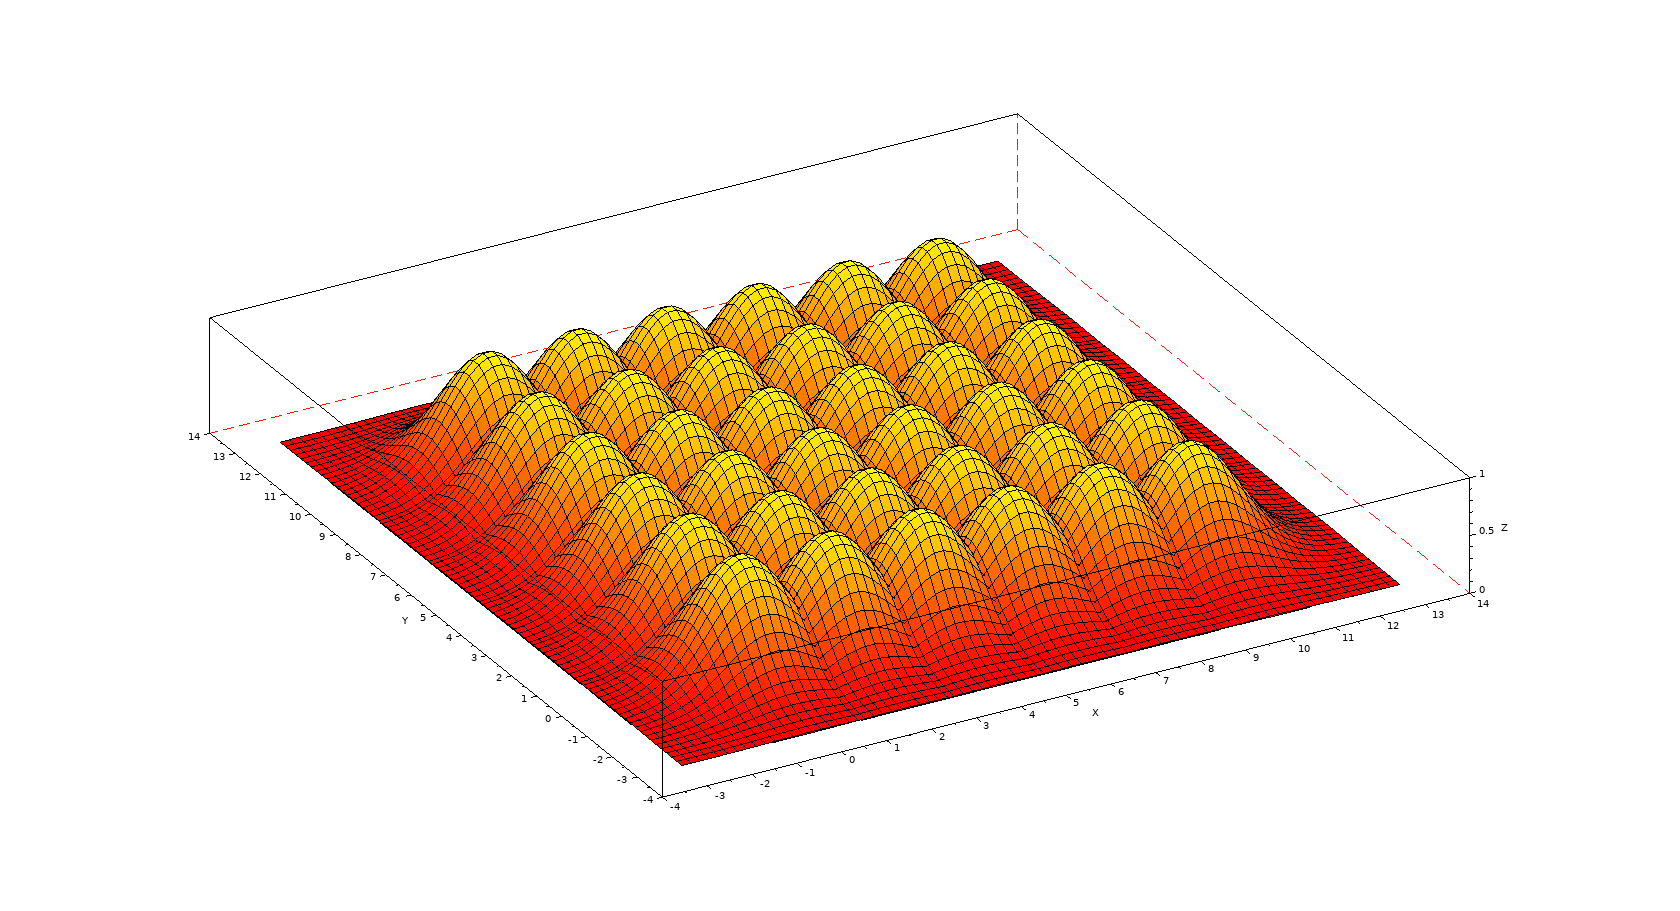
\includegraphics[scale=0.16]{matrixbubblesample.png}
\caption{Visual Representation of a Bubbled Grid\cite{bubble}}
\end{center}
\end{figure}

Then for each square grid, we fit all the points in the square grid to a normal distribution. This reduces all these points to two values ($\mu, \sigma$) that summarize them.

Once we've summarized both matrices $M$ and $N$ to $M'$ and $N'$ with lower dimensions, we can now proceed to compare. As a result of the nature of our reduction (with probability distributions), we cannot simply use any of the regular distance metrics like Euclidean, $L_p$ norm, etc. This is because we could have two normal distributions that are the same but orders of magnitude away from each other by Euclidean distance, etc so we need a theoretical sound way of comparing probability distributions.

Previously, during the midterm project we had implemented a rudimentary version of matrix bubbling to see how well it would work. The initial implementation was fraught with hardship, long execution times, singular matrix errors, negative distances, and unlikely-looking results. In order to remedy that, we improved some aspects of the implementation. One important improvement was to replace the use of the matrix inverse with the Moore-Penrose pseudoinverse wherever a matrix inverse was used. The nature of the data used meant that sometimes, within a bubble it would tend to lie along a single line. This means that the covariance of a certain matrix bubble would be singular. Using the pseudoinverse instead allows us to calculate distances even when the matrix is singular.

\section{Midterm Results}

During the midterm project, we obtained some rudimentary results testing the code on some distorted images. We compared a picture of the letter ``a'' to distorted versions of the same picture, and also to versions of a picture of the letter ``b''. The main result we found was that we needed to fix the problem of non-invertibility of some of the covariance problems, since many of the calculations returned errors. We found that the Hellinger distance, when it didn't error, tended to work better that the KL divergence. The Hellinger distance between the ``a'' and distorted versions of itself was generally smaller than the distance between the ``a'' and the ``b''. This is what we expect, since the ``a'' picture is more similar to itself. The KL divergence, however, performed worse. For reasons currently unknown, the distance between the pictures that should be similar was an order of magnitude larger than the distance between the different pictures. In addition, most of the distances we attempted to calculate ended up giving us errors.

These results led us to believe that the KL divergence likely is not the best option, and that the Hellinger distance would be better to use. However, we needed to fix the problem of singular covariance matrices and test them both again to be sure.

\section{Solutions to Noninvertibility}

\subsection{Moore-Penrose pseudoinverse}

The Moore-Penrose inverse of a matrix is a type of matrix pseudoinverse.\cite{wikimoore} A pseudoinverse of a matrix is a generalization of the inverse matrix. A common use of the pseudoinverse is to compute a ``best fit'' (least squares) solution to a system of linear equations that lacks a unique solution. Another use is to find the minimum (Euclidean) norm solution to a system of linear equations with multiple solutions.

One thing to note is that the pseudoinverse exists and is unique for any matrix. This is useful since inverse matrices do not always exist for matrices. If we wanted to perform calculations that require the inverse of a matrix and we are given a noninvertible matrix, then we would be unable to compute the inverse. As a substitute, we could use the pseudoinverse since the pseudoinverse always exists. One specific example where the inverse of a matrix is required is found in the Hellinger distance.

Consider the following formula for the Hellinger distance between two multivariate Gaussian distributions.

\begin{equation}
    H^2(P,Q)=1-\frac{\det\Sigma_1^{1/4}\det\Sigma_2^{1/4}}{\det \frac{\sigma_1+\sigma_2}{2}^{1/2}}
    \exp\Pn{-\frac18(\mu_1-\mu_2)^T\frac{\sigma_1+\sigma_2}{2}^{-1}(\mu_1-\mu_2)}
\end{equation}

We note that we must compute the inverse of $\Sigma_2$. If $\Sigma_2$ happens not to be invertible, then we will get an error and we will be unable to determine the distance between the two distributions. The Moore-Penrose inverse can be helpful here. Rather than computing the inverse of $\Sigma_2$, we can compute the Moore-Penrose inverse instead, which should serve as a reasonable approximation to the inverse. This is useful for our matrix bubbling project since we require the Hellinger distance to compute the difference between two Gaussian distributions. Using the Moore-Penrose pseudoinverse allows us to compute the Hellinger distance even if $\Sigma_2$ is not invertible.

We first define what the Moore-Penrose inverse of a matrix is. Given any matrix $A$, the Moore-Penrose inverse $A^+$ is a matrix satisfying the following four criteria, known as the Moore-Penrose conditions.

\begin{enumerate}[(a)]
    \item $AA^+A=A$
    \item $A^+AA^+=A^+$
    \item $(AA^+)^*=AA^+$
    \item $(A^+A)^*=A^+A$
\end{enumerate}

Again, $A^+$ exists for any matrix $A$, even if $A$ is not invertible. One thing worth noting is that when $A$ has linearly independent columns (and thus the matrix $A^*A$ is invertible), $A^+$ can be computed as
\[
    A^+=(A^*A)^{-1}A^*.
\]
In the case that $A$ is a square matrix, which it will be in the case that we are considering, then if it is invertible, the Moore-Penrose pseudoinverse is just the inverse of the matrix, as expected.

The Moore-Penrose inverse can also be characterized in terms of the singular value decomposition. Suppose that the matrix $A$ is decomposed as
\[
    A=U\Sigma V^*.
\]
If the matrix $A$ is invertible, then $A^{-1}=V\Sigma^{-1}U^*$. This will occur if there are no non-zero singular values. In that case, $\Sigma$ is a diagonal matrix with entries $\sigma_i$, and $\Sigma^{-1}$ is a diagonal matrix with entries $\sigma_i^{-1}$.

If $\Sigma$ is not invertible, that is, there are some singular values equal to $0$, the pseudoinverse $\Sigma^+$ is formed by replacing each non-zero singular value $\sigma_i$ by $\sigma_i^{-1}$, while keeping each zero singular value as $0$. In that case, it is easily seen that $\Sigma$ and $\Sigma^+$ satisfy the requirements for the Moore-Penrose pseudoinverse above. Moreover, the pseudoinverse of $A$ is given by $A^+=V\Sigma^+U^*$. As an example, for the first property, we have
\begin{align*}
    AA^+A&=(U\Sigma V^*)(V\Sigma^+ U^*)(U\Sigma V^*)\\
    &=U(\Sigma\Sigma^+\Sigma)V^*\\
    &=U\Sigma V^*\\
    &=A
\end{align*}

\subsection{Perturbation of singular matrices}

Another way that singular matrices can be dealt with is by perturbing them slightly. Doing so will almost certainly convert a singular matrix to a non-singular matrix, assuming that the perturbation is random. This occurs because of the density of invertible matrices in the set of all matrices. In fact, the set of singular matrices is a lower-dimensional submanifold of the set of all matrices. This is because the requirement for a matrix to be singular, $\det A=0$, is a smooth function from the set of matrices to $\mathbb R$. Its zero set, then, should be a closed submanifold of codimension $1$. For $2\times 2$ matrices representing covariance of $2$-dimensional data, the set of all matrices is $4$-dimensional while the singular matrices are a $3$-dimensional submanifold.

However, even though perturbing a singular matrix slightly can make it non-singular, there are a couple reasons why it is not the best option. One is that the resulting matrix, while non-singular, will still be close to singular. It can be inverted, but matrices that are almost singular (and so the determinant is almost zero) can cause some problems, especially numerically.

This leads to the other problem, where the perturbation can drastically change the distance that we get. This is because the inverse may be quite different. For example, suppose that the original (singular) matrix is $A$. One possible way to perturb the matrix would be to add a multiple of the identity to it. Since $A$ is singular, it has $0$ as an eigenvalue. If we restrict $A$ to the generalized eigenspace of eigenvalue $0$, and say the restriction is $A'$, then $A'$ will be nilpotent. In that case, $A'^n=0$ for some $n$. Then by direct multiplication, we can see that
\[
    (\epsilon I+A')(\epsilon^{-1}I-\epsilon^{-2}A'+\epsilon^{-3}A'^2-\cdots
    \pm\epsilon^{-n}A'^{n-1})=I.
\]
Since changing $\epsilon$, for small $\epsilon$, creates big differences in the inverse of $A'+\epsilon I$, this method would not lead to consistent results. Because of these problems, we decided that the best option would be to use the pseudo-inverse to avoid having problems with singular matrices.

\subsection{Distance metrics}

When measuring the distance between two probability distributions, there are several distance functions that could be used. After looking at some different options during our midterm project, the two that we decided were best to focus on are the Hellinger distance and the KL divergence. Both of those distances have the issue that they don't have a closed form for most general probability distributions, and have to be integrated numerically. Fortunately, for the normal distribution, a closed-form expression can be derived for both the Hellinger distance and the KL divergence. This makes the normal distribution especially nice to work with, and is one of the reasons that we decided to use the normal distribution to approximate the probability distributions in the images.

\subsubsection{Hellinger Distance}

The Hellinger distance is one measure of a distance from one probability distribution to another.\cite{wikihell} It is a metric, meaning that it is symmetric and satisfies the triangle inequality. The Hellinger distance between two probability distributions is given by
\[
    H^2(P,Q)=1-\int \sqrt{f(x)g(x)}\,dx.
\]
Note that the Hellinger distance is always between $0$ and $1$. For multivariate normal distributions $P$ and $Q$, where $P$ has mean $\mu_1$ and covariance matrix $\Sigma_1$ and $Q$ has mean $\mu_1$ and covariance matrix $\Sigma_2$, the Hellinger distance is given by \cite{pardo}
\begin{multline*}
    H^2(P,Q)=1-\frac{\det\Sigma_1^{1/4}\det\Sigma_2^{1/4}}
    {\det\Pn{\frac{\Sigma_1+\Sigma_2}{2}}^{1/2}}\\
    \exp\Pn{-\frac18(\mu_1-\mu_2)^T\Pn{\frac{\Sigma_1+\Sigma_2}{2}}^{-1}
    (\mu_1-\mu_2)}.
\end{multline*}
Although this expression is undefined when $\frac{\Sigma_1+\Sigma_2}{2}$ is singular, the distance itself is still well-defined in that case (the formula just doesn't apply as written).

\subsubsection{KL Divergence}

The KL divergence is a measure of how much one probability distribution ``diverges'' from another.\cite{wikikl} Given a probability distribution $P$ and another distribution $Q$, the KL divergence from $P$ to $Q$ can be thought of as a measure of how well the distribution $Q$ approximates $P$. That is, if $P$ is the actual distribution, and $Q$ is some distribution that is intended to approximate $P$, then the KL divergence measures how good of an approximation $Q$ is. It is defined by
\[
    D_{KL}(P\| Q)=\int_{-\infty}^\infty p(x)\log\Pn{\frac{p(x)}{q(x)}}\,dx,
\]
where $p(x)$ and $q(x)$ are the probability density functions of $p$ and $q$. For two normal distributions, this distance works out to be
\begin{align*}
    D_{KL}(P\| Q)
    &=\frac12\Pn{\log\frac{\det\Sigma_2}{\det\Sigma_1}+\Delta\mu^T\Sigma_2^{-1}\Delta\mu+\Tr(\Sigma_1\Sigma_2^{-1})-n},
\end{align*}
where $\Delta\mu$ is the difference between the mean vectors, $\Sigma_1$ is the covariance vector for $P$, and $\Sigma_2$ is the covariance vector for $Q$. We can see from the formula that this expression is undefined when $\Sigma_2$ is singular. This issue is worse than in the Hellinger distance case, because the distance itself is undefined in that case. For the KL divergence to be defined, it is necessary that $Q$ have a non-zero probability on every set where $P$ has a non-zero probability. Therefore if the covariance matrix for $Q$ is not full rank, the KL divergence from $P$ to $Q$ will be infinite. (This happens because $Q$ is supposed to approximate the actual probability distribution $P$. If we use $Q$ as the approximation, and $Q$ has a $0$ probability on some set, then we would expect that never to happen. If $P$ then has a positive probability, then in reality there is a positive probability that it will happen, which we would be infinitely surprised about if we expect the probability to be $0$.)

Unlike the Hellinger distance, the KL divergence is not a metric; it is not symmetric. When doing tests, we distinguish between a certain complete base image, and a set of test images; we want to determine if each test image matches the base image. For our purposes, then, we use the base image distribution as $P$, and the test images as $Q$.

\section{Methods}

For each image, we compute the matrix bubble as follows. We take the image and break it into blocks of $n$ by $n$ submatrices, or bubbles. For each of these bubbles, we compute the mean and covariance matrix as follows. For each coordinate $(x, y)$ in the bubble, we take its intensity value $n$ and we add $n/5$ copies of $(x, y)$ to an array. (We divide by 5 so we have fewer elements in our array. It is reasonable since two pixel values that are within 5 of each other are very hard to distinguish.) We then compute the mean and covariance matrix, which is two-dimensional.

Then, given two matrix bubbles of two images, we need a way to find the distance between them. This is accomplished by finding the distance between each bubble, and then combining the distance of all the bubbles. The distance between two bubbles was found using one of the statistical distances, either the Hellinger distance or the KL divergence. Once we have a distance $d$ that computes the distance between two bubbles, the total distance between the matrices is given as the $L^1$ norm of the bubble distances. If $P_{ij}$ are the bubbles of the first matrix and $Q_{ij}$ are the bubbles of the second, then the total distance is given by
\[
    \sum_{i,j} d(P_{ij},Q_{ij}).
\]
It is possible that some bubbles would not have any data in them, which could be because the data is missing or otherwise does not exist in that area. In that case, there is no distribution for that bubble, so it is not included in the sum to calculate the total distance. In other words, the distance is 0. In addition to combining all of the data into a single number for the distance, we can also look at the distance between each of the bubbles. This gives an idea of where the picture is similar and where it is different, and we plotted the distance as a heatmap over the image in order to see how much it differs in different areas and whether that agrees with what we would expect the distance to be.

\subsection{Distorted Letters}

We tested this first on black-and-white pictures of cursive letters.\cite{alphabetsprintables}

\begin{figure}[h!]
\begin{center}
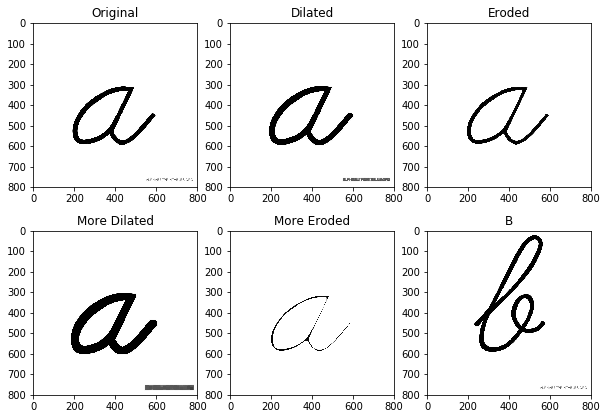
\includegraphics[width=0.7\textwidth]{a.png}
\caption{Sample Cursive Letters}
\label{fig:letters}
\end{center}
\end{figure}

Figure \ref{fig:letters} shows the pictures of the letters that were used. Starting with the letter ``a'', we distorted it using various morphological operators.\cite{morph}\cite{dilation} One such operator is erosion, where each pixel is replaced with the brightest of the surrounding pixel values. This has the effect of taking the dark letter and making it thinner. The other operator we tried was dilation, which replaces each pixel with the darkest of the surrounding values. This causes the dark letter to become thicker. Finally, we also used a picture of a different letter, ``b''. If the matrix bubbling method works as desired, we would hope that the distance between the original ``a'' and the modified ``a''s is smaller than the distance from the ``a'' to the ``b''.

\subsection{Compressed Dogs}

The other type of distortion that we analyzed was image compression. We started with a grayscale picture of a dog, and compared the original image with various compressed images. In order to perform the compression, we used the singular value decomposition method of compression. The steps of this method are to start with the image, and compute its singular value decomposition. Then to compress the image, we save only the data associated to the first $N$ singular values for different values of $N$, producing a rank $N$ approximation to the original image. Figure \ref{fig:doggos} shows the dog picture and the various compressed versions. We would expect the distance from the original picture to each of the compressed versions to increase the more the picture is compressed, that is, the lower the rank of the image.

\begin{figure}[h!]
\begin{center}
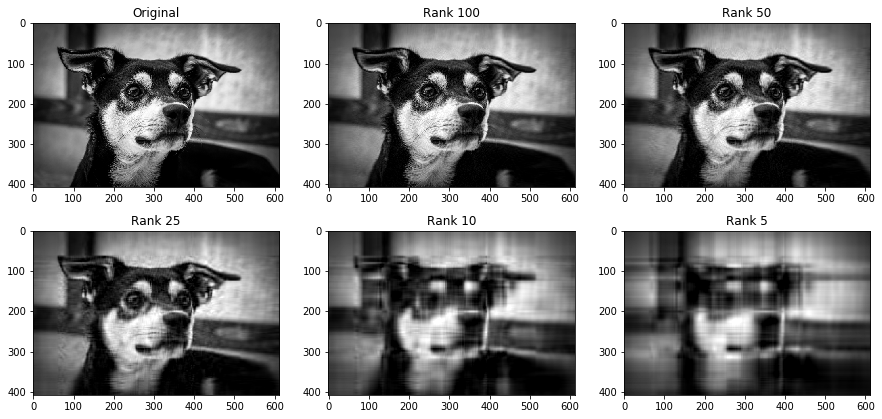
\includegraphics[width=\textwidth]{dogs.png}
\caption{Compressed Dog Images}
\label{fig:doggos}
\end{center}
\end{figure}

Another thing we experimented with was the bubble size. We used bubble sizes of $n=15$, $n=30$, and $n=50$ to see how bubble size affected the distances.

\section{Results}

We analyze our results below.

\subsection{Distorted Letters}

\begin{figure}[h!]
\begin{center}
\begin{tabular}{ c || c | c | c | c | c | c }
    & Original & Dilated 1 & Eroded 1 & Dilated 2 & Eroded 2 & B \\ \hline
    Hell & 0.00 & 37.54 & 31.86 & 83.72 & 57.52 & 65.11 \\
    KL & 0.00 & 268.21 & 113.78 & 2584.99 & 241.87 & 2786.87
\end{tabular}
\caption{Comparison of Distorted Letters ($n=15$)}
\label{fig:a15}
\end{center}
\end{figure}

\begin{figure}[h!]
\begin{center}
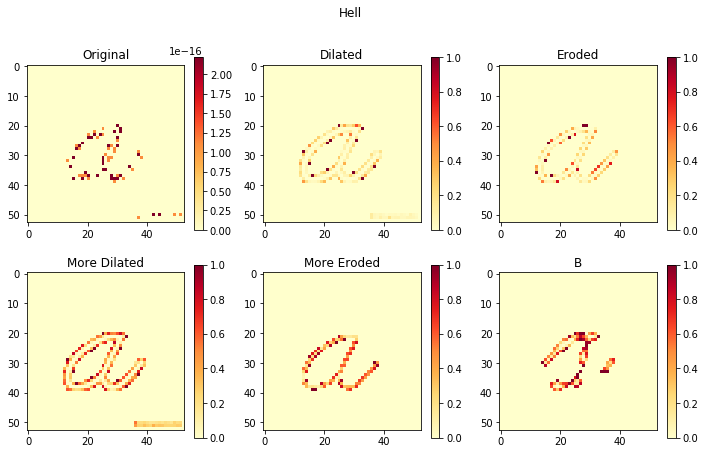
\includegraphics[width=0.7\textwidth]{hell-a.png}
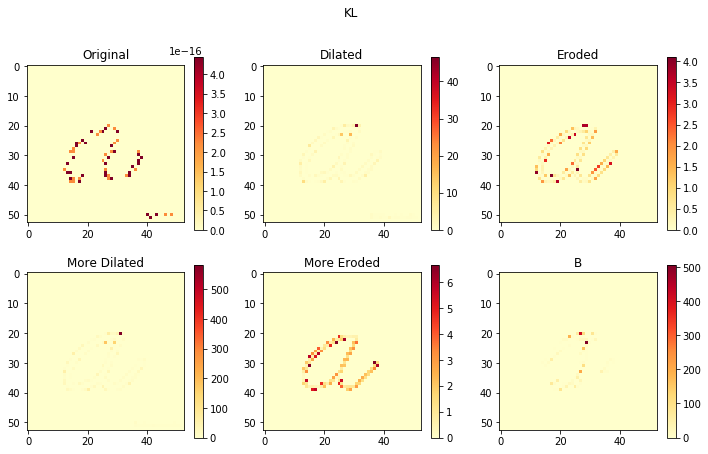
\includegraphics[width=0.7\textwidth]{kl-a.png}
\caption{Heatmap of Distorted Letters}
\label{fig:aheat}
\end{center}
\end{figure}

Figure \ref{fig:a15} shows the results for the distances between the letter ``a'' and the various distortions, as well as the letter ``b''. We can see that the Hellinger distances and KL divergences behave similarly, although the absolute values of the KL divergences are larger. For the small changes, slight dilation and slight erosion, the distance from the ``a'' are smaller than the distance to the ``b'', so the method is working as intended. For the larger changes, the distances are comparable to the ``b'', so the method does not work that well when the distortion is too significant. Looking at the picture used, it does not seem too surprising that the significantly dilated and eroded ``a''s would have such a large distance, since there is a lot of black either added or taken away, and the bubbles are small enough that the method does not capture the general shape features as a whole. We can see in the heatmap, Figure \ref{fig:aheat}, that the differences tend to be at the border of the ``a'', where black is added or removed, which is what we would expect.

\subsection{Compressed Dogs}

\begin{figure}[h!]
\begin{center}
\begin{tabular}{ c || c | c | c | c | c }
    & Rank 100 & Rank 50 & Rank 25 & Rank 10 & Rank 5 \\ \hline
    Hell & 18.09 & 17.60 & 25.33 & 35.25 & 49.37 \\
    KL & 1370.65 & 1312.01 & 1432.93 & 1265.56 & 1792.24
\end{tabular}
\caption{Comparison of Compressed Dogs ($n=15$)}
\label{fig:dog15}
\end{center}
\end{figure}

\begin{figure}[h!]
\begin{center}
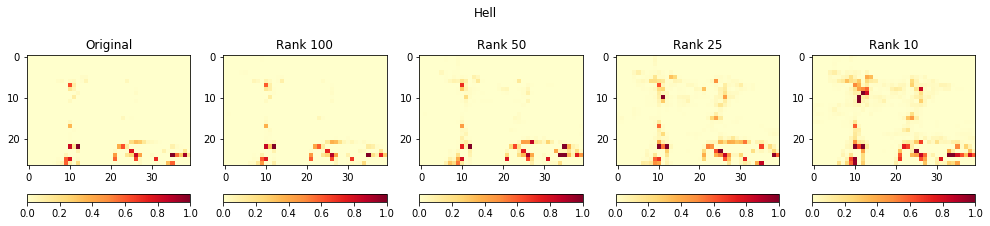
\includegraphics[width=\textwidth]{hell-dogs-15.png}
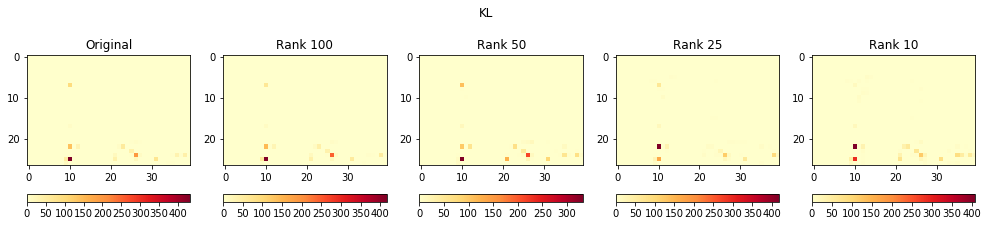
\includegraphics[width=\textwidth]{kl-dogs-15.png}
\caption{Heatmap of Compressed Dogs ($n=15$)}
\label{fig:dogheat15}
\end{center}
\end{figure}

For the dog pictures, the comparison of the original dog to the compressed versions is shown in Figure \ref{fig:dog15}. We see that as the image gets more compressed, the distance generally goes up, with a couple exceptions. We also tried increasing the bubble size from 15 to 30 (shown in Figure \ref{fig:dog30}), and even more to 50 (shown in Figure \ref{fig:dog50}). The Hellinger distance behaves pretty well, consistently increasing as the image is compressed more. The KL divergence is a little more wild. In all cases, the total distance is smaller when the bubbles are larger because there are fewer bubbles, and the total distance is the sum of the individual bubble distances.

\begin{figure}[h!]
\begin{center}
\begin{tabular}{ c || c | c | c | c | c }
    & Rank 100 & Rank 50 & Rank 25 & Rank 10 & Rank 5 \\ \hline
    Hell & 4.21 & 5.23 & 5.55 & 7.86 & 13.44 \\
    KL & 606.58 & 1196.57 & 1306.57 & 294.02 & 1512.20
\end{tabular}
\caption{Comparison of Compressed Dogs ($n=30$)}
\label{fig:dog30}
\end{center}
\end{figure}

\begin{figure}[h!]
\begin{center}
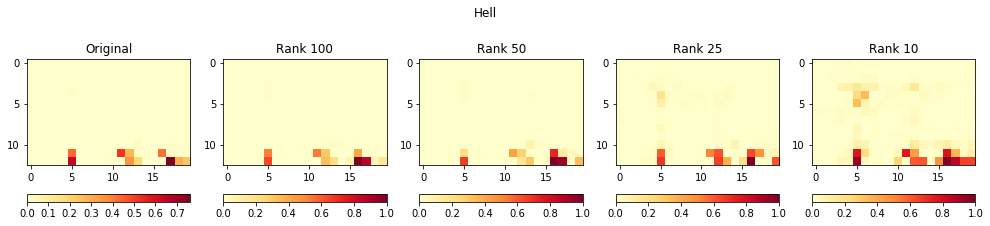
\includegraphics[width=\textwidth]{hell-dogs-30.png}
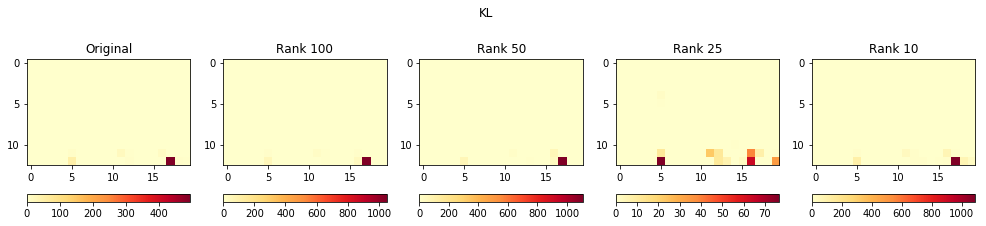
\includegraphics[width=\textwidth]{kl-dogs-30.png}
\caption{Heatmap of Compressed Dogs ($n=30$)}
\label{fig:dogheat30}
\end{center}
\end{figure}

The reason that the KL divergence is so much more variable is likely because it is unbounded, and can go anywhere from 0 to infinity. Thus a single bubble which is especially different under the KL divergence will cause a large outlier and greatly affect the distance as a whole. This seems like an overall undesirable category, so the Hellinger distance is probably a better option, since it is bounded to be between $0$ and $1$ for each bubble.

\begin{figure}[h!]
\begin{center}
\begin{tabular}{ c || c | c | c | c | c }
    & Rank 100 & Rank 50 & Rank 25 & Rank 10 & Rank 5 \\ \hline
    Hell & 0.59 & 0.63 & 0.81 & 2.32 & 3.63 \\
    KL & 5.75 & 5.48 & 6.00 & 28.94 & 45.89
\end{tabular}
\caption{Comparison of Compressed Dogs ($n=50$)}
\label{fig:dog50}
\end{center}
\end{figure}

\begin{figure}[h!]
\begin{center}
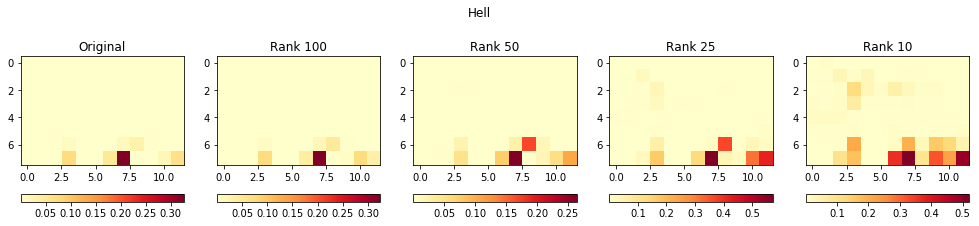
\includegraphics[width=\textwidth]{hell-dogs-50.png}
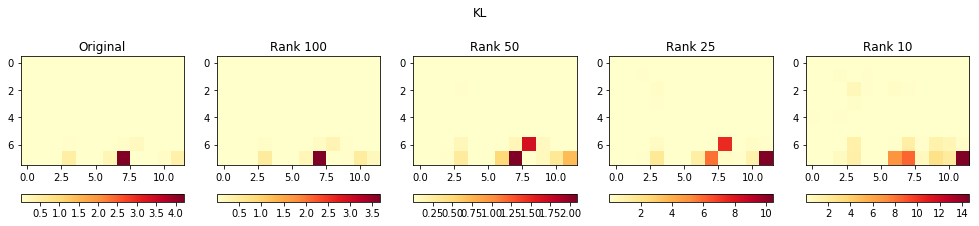
\includegraphics[width=\textwidth]{kl-dogs-50.png}
\caption{Heatmap of Compressed Dogs ($n=50$)}
\label{fig:dogheat50}
\end{center}
\end{figure}

The variability is visible in the heatmaps, as well. For the Hellinger distance, the heatmap has more of a continuous range of variability, and there are many spots that are clearly darker, showing the areas that are more different, and some that are lighter. For the KL divergence, there tend to be a few very dark spots, and the rest are all light, suggesting that the the total distance in that case is all coming from just a small number of outlier bubbles.

\clearpage
\printbibliography
\end{document}
